\documentclass[11pt,a4paper]{article}
\usepackage[catalan]{babel}

% Paquetes necesarios
% preamble.tex

% Codificación y tipografía
\usepackage[utf8]{inputenc}
\usepackage[T1]{fontenc}
\usepackage[catalan]{babel}
\usepackage{lmodern}

% Márgenes y geometría
\usepackage{geometry}
\geometry{left=2.5cm, right=2.5cm, top=2cm, bottom=3cm}
% Estilo de página
\usepackage{fancyhdr}
\setlength{\headheight}{15pt}
\pagestyle{fancy}
\fancyhf{}
\lhead{\textit{Electrònica Física}}
\rhead{\textit{Adrià Rojo}}
\cfoot{\thepage}

% Gráficos y tablas
\usepackage{graphicx}
\usepackage{float}
\usepackage{caption}

% Matemáticas y símbolos
\usepackage{amsmath}
\usepackage{amssymb}

% Hipervínculos
\usepackage{hyperref}

% Espaciado
\usepackage{parskip}  % Quita sangría de párrafos y añade espacio
\usepackage{wrapfig}
\usepackage[backend=biber,style=ieee, autocite=superscript]{biblatex}
\addbibresource{bibliography.bib}

% Fuente y estilo general
\renewcommand{\familydefault}{\rmdefault}

%Definició de la ela geminada per tal que accepti el punt volat del teclat
% \def·#1{%
%   \ifmmode
%     \cdot #1
%     %\csname normal@char\string"\endcsname l%
%   \else%
%     \def\argument{#1}%
%     \if\argument l%
%       \leftllkern=0pt\rightllkern=0pt\raiselldim=0pt%
%       \setbox0\hbox{l}\setbox1\hbox{l\/}\setbox2\hbox{.}%
%       \advance\raiselldim by \the\fontdimen5\the\font
%       \advance\raiselldim by -\ht2%
%       \leftllkern=-.25\wd0%
%       \advance\leftllkern by \wd1%
%       \advance\leftllkern by -\wd0%
%       \rightllkern=-.25\wd0%
%       \advance\rightllkern by -\wd1%
%       \advance\rightllkern by \wd0%
%       \allowhyphens\discretionary{-}{l}%
%       {\hbox{}\kern\leftllkern\raise\raiselldim\hbox{.}%
%         \kern\rightllkern\hbox{l}}\allowhyphens%
%     \else
%       \if\argument L%
%         \leftllkern=0pt\rightllkern=0pt\raiselldim=0pt%
%         \setbox0\hbox{L}\setbox1\hbox{L\/}\setbox2\hbox{.}%
%         \advance\raiselldim by .5\ht0%
%         \advance\raiselldim by -.5\ht2%
%         \leftllkern=-.125\wd0%
%         \advance\leftllkern by \wd1%
%         \advance\leftllkern by -\wd0%
%         \rightllkern=-\wd0%
%         \divide\rightllkern by 6%
%         \advance\rightllkern by -\wd1%
%         \advance\rightllkern by \wd0%
%         \allowhyphens\discretionary{-}{L}%
%         {\hbox{}\kern\leftllkern\raise\raiselldim\hbox{.}%
%            \kern\rightllkern\hbox{L}}\allowhyphens%
%       \else
%         #1
%       \fi
%     \fi
%   \fi
%   }
% Título
\title{\textbf{CMOS: Història, fonaments i funcionament digital i aplicacions}}
\author{Adrià Rojo}
\date{\today}

\begin{document}

\maketitle
\thispagestyle{empty}
% Resumen
\begin{abstract}
La tecnologia \textit{Complementary-Metal-Oxide Semiconductor} (CMOS) és la base de la microelectrònica moderna gràcies al seu baix consum energètic, alta densitat d'integració i eficàcia en circuits digitals. Aquest treball presenta una visió general de la seva evolució al llarg dels anys, des dels primers transistors MOSFET fins a la consolidació de la lògica CMOS com a estàndard industrial. A més, s'analitza el funcionament intern dels transistors nMOS i pMOS, amb especial atenció a la formació del canal, les condicions de conducció i el comportament digital dels dispositius. S'expliquen també estructures lògiques com la porta NOT i NAND, i es mostren aplicacions actuals del CMOS, com poden ser processadors o sensors d'imatge. El treball es centra en una descripció funcional digital, deixant de banda els models analògics, amb l’objectiu d’entendre per què el CMOS segueix sent fonamental en la tecnologia electrònica contemporània.
\end{abstract}


\section{Introducció}
% Introducir brevemente qué es CMOS, su importancia en la electrónica digital y qué estructura tendrá el trabajo.

Un semiconductor-òxid-metall complementari (\textit{Complementary-Metal-Oxide Semiconductor}) o CMOS, és un tipus de tecnologia que combina un parell simètric de nMOS i pMOS connectats de forma complementària per poder fer operacions lògiques de forma eficient\autocite{wiki:CMOS}. 

Aquesta tecnologia és la base d'electrònica moderna, sent el bloc principal de la porta lògica \texttt{NAND}, que és la base de tots els altres circuits existents i pot arribar formar circuits molt complexos com processadors i memòries RAM.

Els dispositius dissenyats amb el procés CMOS en ment també poden ser utilitzats com a sensor d'imatge, gràcies a la seva eficiència i rapidesa, formant part d'una àmplia varietat d'eines electròniques, des de telèfons mòbils a drons i càmeres fotogràfiques utilitzades en medicina o astronomia. 

Actualment s'estima que el nombre de transistors MOSFET manufacturats (inclou els CMOS) superen els $10^{22}$ dispositius \autocite{wiki:Transistor_count} el 2018, dada que està basada en la Llei de Moore.

A continuació, repassarem la història del CMOS, analitzarem els principis físics i el seu funcionament intern, especialment orientat a l'electrònica digital, i explorarem les seves aplicacions actuals i futures, mostrant perquè continua sent una tecnologia essencial en el desenvolupament tecnològic modern.

\section{Història del CMOS}
% Destacar los hitos importantes desde 1963, comparaciones con tecnologías anteriores (nMOS, BJT).
% Mencionar su adopción masiva en los años 80-90 y cómo ha evolucionado.

\subsection{BJT i MOSFET}


Al final dels anys 1940, el transistor bipolar de junció, o BJT, va ser inventat per John Bardeen i Walter Brattain sota la direcció de William Shockley als laboratoris Bell Telephone. Gràcies a certes millores introduïdes de cara a l'eficiència, tant en el seu ús com a la seva producció, van ser introduïts al públic general als principis dels anys 1950 i van ser la tecnologia predominant al mercat durant trenta anys.

\begin{wrapfigure}{r}{0.25\paperwidth}
    \centering
    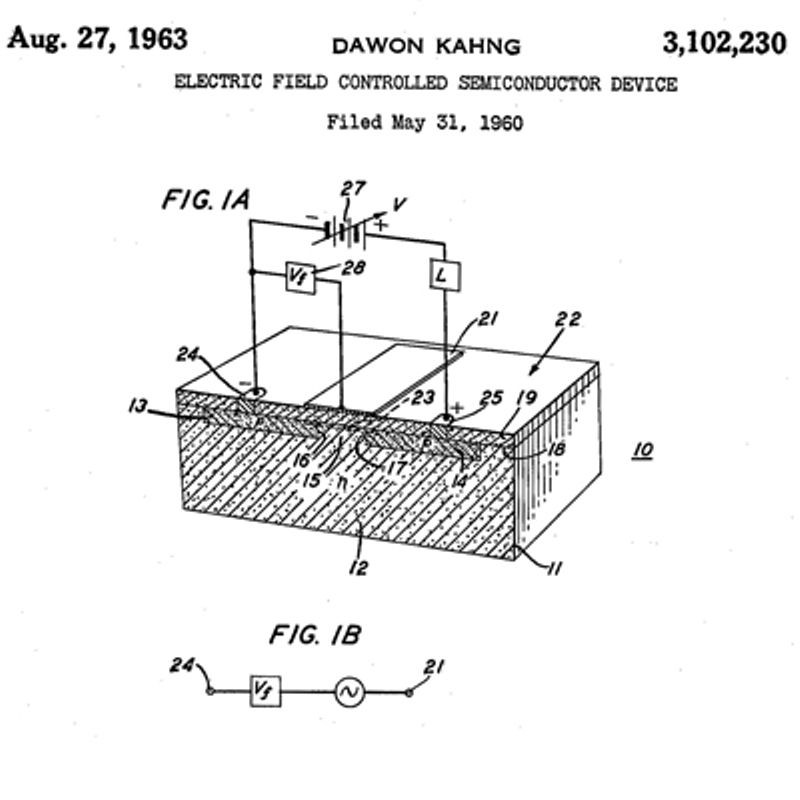
\includegraphics[width=\linewidth]{images/patent kahang.jpg}
    \caption{Patent \texttt{US3102230A} estatunidenca del MOSFET de Dawon Kahng.}
    \vspace{-1.4cm}
\end{wrapfigure}
Prèviament, el transistor d'efecte de camp semiconductor-òxid-metall, o MOSFET, ja s'havia inventat i patentat a Europa. Aquest va ser objecte d'estudi per part de l'equip dels laboratoris Bell, però sense èxit, a causa dels problemes dels estats superficials \footnote{Els estats superficials són els estats electrònics que es formen a la superfície dels materials, deguts a la interrupció de la malla atòmica del material que acaba en la superfície. Aquest efecte es pot pal$\cdot$liar amb la \textit{passivització} de la superfície, que redueix l'efecte i estabilitza els estats electrònics al límit del material.} no va ser possible la seva adopció a gran escala.

Després d'avenços amb el transistor (òxid de Silici com a passivitzador, invenció de la tecnologia de fabricació planar), finalment Mohamed Atalla i Dawon Kahng van introduir el primer transistor MOS de silici funcional als laboratoris Bell l'any 1960. 

Tot i això, els transistors MOSFET no estaven a l'altura dels BJT de l'època i eren vistos com a inferiors. La principal diferència entre els MOSFET i BJT és el consum elèctric i el seu ús típic: 
\\
\begin{itemize}
    \item Els BJT són controlats per corrent a la base, i aquest corrent controla el flux entre el col·lector i l'emissor. Tenen un comportament lineal i són ideals per a circuits analògics. Requereixen un flux de corrent constant per funcionar.
    \item Els MOSFET, quan s'utilitzen en configuració CMOS, només consumeixen energia durant els canvis d'estat (commutació), cosa que els fa especialment adequats per a circuits digitals. Fora de CMOS, els MOSFET pMOS i nMOS per separat també poden consumir energia de forma contínua segons com estiguin polaritzats.
\end{itemize}


El primer circuit integrat amb tecnologia MOSFET (únicament pMOS) va ser presentat al 1964 per General Microelectronics i el primer aparell d'us quotidià (una calculadora) amb aquests circuits va ser presentada per la mateixa empresa un any després\autocite{general_microelectronics}.
\begin{wrapfigure}{r}{0.2\paperwidth}
    \centering
    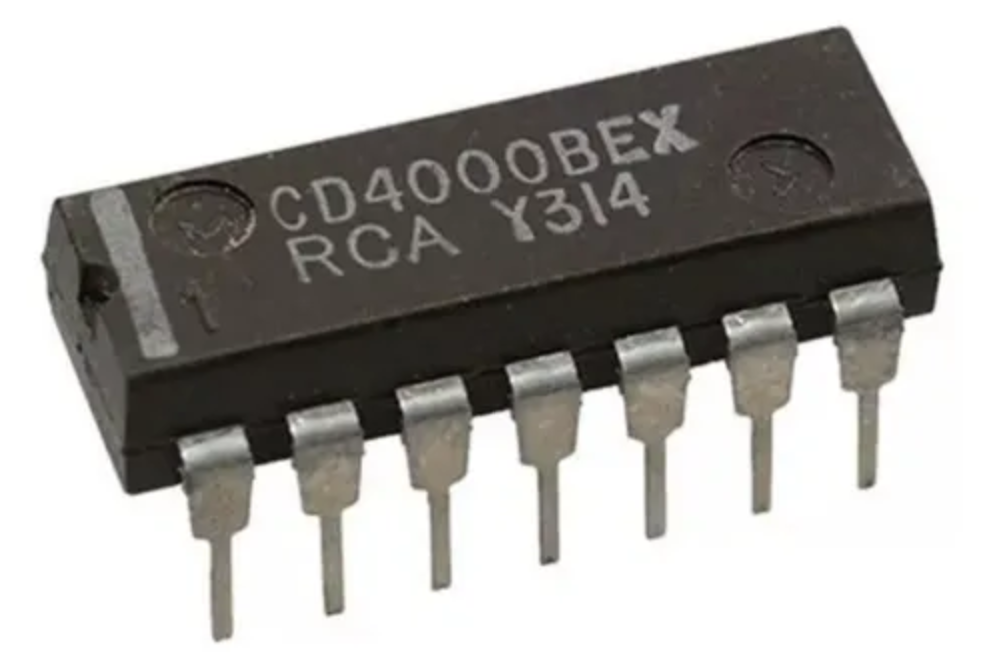
\includegraphics[width=\linewidth]{images/rca cd4000 chip.png}
    \caption{Xip de la família CD4000 de RCA.}
    \vspace{-1.3cm}
\end{wrapfigure}

\subsection{Naixement del CMOS, primers dispositius}

A mesura que augmentava la densitat dels circuits integrats, el consum energètic i la dissipació tèrmica eren limitacions greus. Això va motivar la recerca de tecnologies més eficients, i el CMOS va ser presentat com una solució prometedora el 1960 per la companyia Fairchild Semiconductor, tenint el seu primer contacte amb el públic el 1968 amb la presentació del xip lògic general CD4000 per RCA\autocite{wiki:4000-series_integrated_circuits}.

Del 1960 al 1980 va ser acceptat de forma àmplia, però van trobar problemes, entre ells un a causa de l'ús dels pMOS dins del CMOS, on els forats són els portadors i la seva mobilitat és inferior a la dels electrons ($\mu_e = \qty{1400}{\centi\meter\squared\per\volt\per\second} \gg \mu_h = \qty{450}{\centi\meter\squared\per\volt\per\second}$), fent reduir la velocitat d'operació del dispositiu. Aquesta limitació va fer sorgir altres alternatives com tecnologia Lògica d'Injecció Integrada, o I$^2$L i al principi dels anys 1980 hi havia una previsió de que CMOS seria desbancat pels mateixos dispositius I$^2$L. 

Però gràcies a la millora en la síntesi dels materials i litografia van poder fer integrar més dispositius CMOS en menys espai (complint així la Llei de Moore). També va arribar un punt on la fabricació de CMOS no era més difícil que la fabricació nMOS, fent així que es consolidés aquesta tecnologia.

\subsection{Actualitat}

Amb el pas del temps, aquesta tecnologia (en general els MOSFET) ha acabat sent una part fonamental de la vida de molta gent, en concret els CMOS ho han sigut a causa del seu baix consum i la seva alta densitat i facilitat de disseny i fabricació. 

Alguns dels dispositius més notables construïts amb aquesta tecnologia són:
\begin{itemize}
    \item Microprocessadors PowerPC de la família 600. En especial el xip PowerPC 620, sent dels primers en treballar en arquitectura de 64 bits.
    \item Microprocessadors Intel de la gamma 8000 i 80000, que utilitzen tecnologia CHMOS, culminant en l'arxiconegut processador Intel Pentium (que utilitza CMOS bipolars de $\qty{800}{\nano\meter}$).
    \item La consola Nintendo Wii, on el seu microprocessador \textit{Hollywood} està fabricat amb tecnologia CMOS de $\qty{90}{\nano\meter}$.
\end{itemize}

\section{Funcionament intern}


\begin{wrapfigure}{r}{0.25\paperwidth}
    \centering
    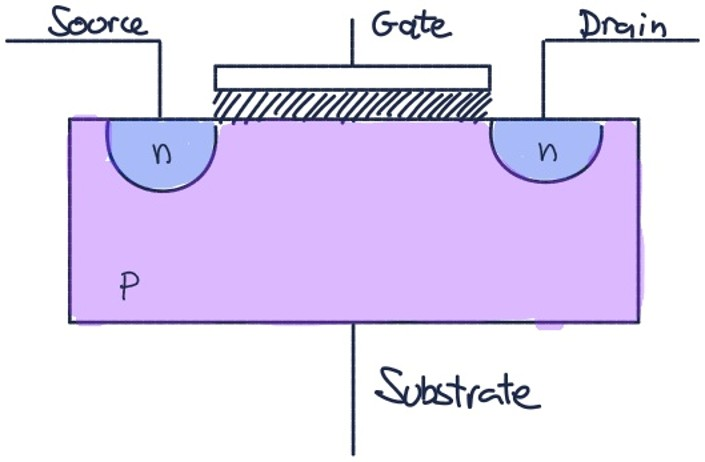
\includegraphics[width=\linewidth]{images/nmos1.jpg}
    \caption{Estructura d'un NMOS}
    \label{fig:nmos1}
    \vspace{-1cm}
\end{wrapfigure}
Els CMOS es basen en tot el funcionament darrere dels MOSFET de tipus P i N. La complementació dels dos dispositius ens permet començar a operar funcions lògiques en un circuit digital.

\subsection{Formació del canal}

El fet diferenciador del CMOS no es pot explicar si no és amb el treball fet pels p i n MOS. Mirarem únicament el nMOS, el pMOS tindrà un funcionament exactament igual, però complementari.

Un dispositiu nMOS (Figura \ref{fig:nmos1}) consta de 4 contactes: Font, Drenatge, Substrat i Porta. L'estructura del nMOS és de la concatenació de semiconductors NPN amb un òxid format sobre el semiconductor P (que seria el substrat) amb un metall a l'altra banda de l'òxid. Aquest òxid i metall amb el semiconductor és el que dona el nom de MOS. Com a tal, l'estructura de substrat-òxid-metall, actuarà com un condensador elèctric, amb una tensió de ruptura associada.

Estant en equilibri entre el D i S ($V_D - V_S = V_{DS} = \qty{0}{\volt}$) si apliquem un voltatge més gran que el voltatge d'umbral o \textit{Threshold voltage}, característic del transistor (depen del semiconductor, amplada, òxid...), entre la porta i substrat hi haurà un camp elèctric localitzat entre aquests. Això farà que els electrons que venen des del contacte del substrat viatgin cap a la porta, però seran interromputs per l'òxid, que és aïllant. L'acumulació d'electrons a la interfície entre el substrat i l'òxid crearà un pont (n-channel) entre els semiconductors de Font i Drenatge.


\begin{figure}[h]
    \centering
    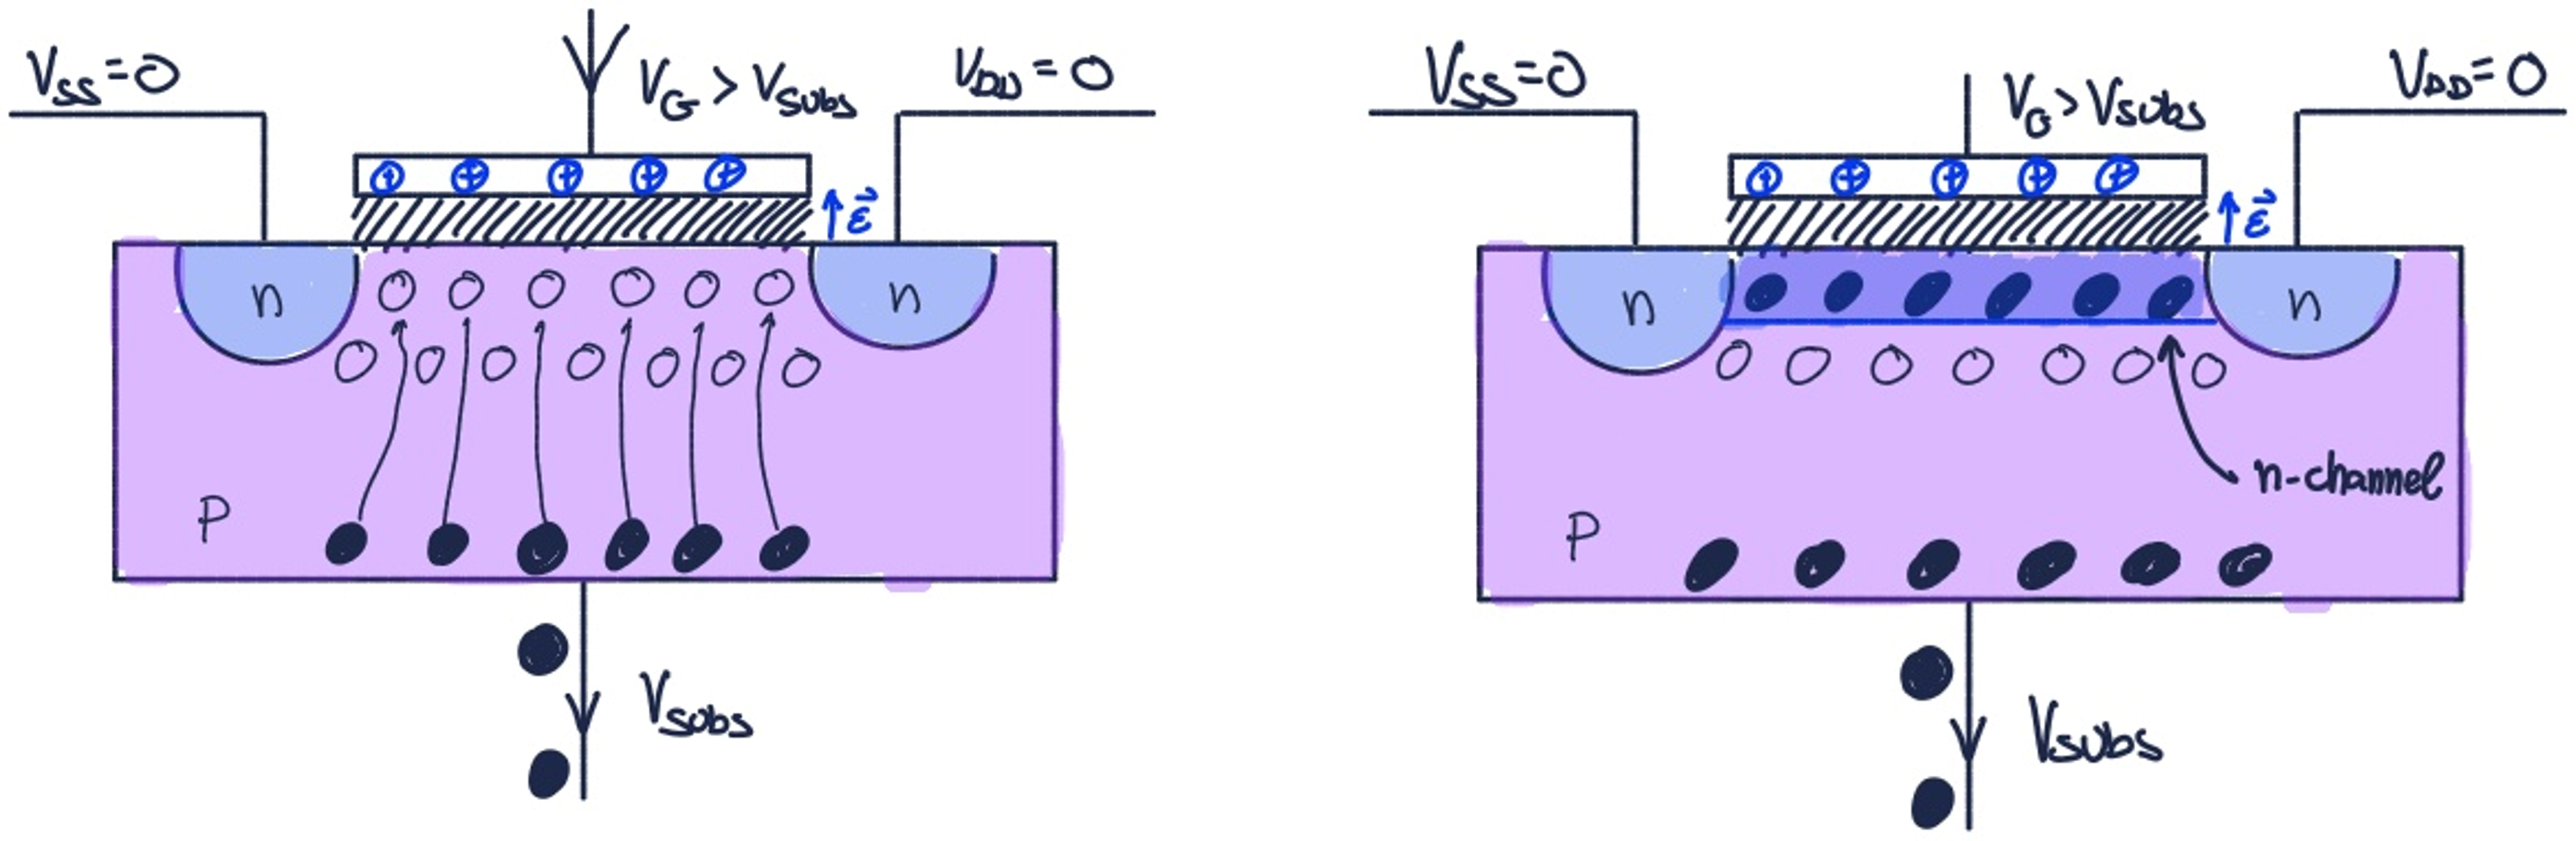
\includegraphics[width=0.6\paperwidth]{images/nmos23.png}
    \caption{Formació del canal en equilibri a $V_D$ = $V_S$}
    \label{fig:nmos23}
\end{figure}

Habitualment els dispositius MOSFET connecten el Substrat amb el Source. Ara bé, quan volem fer passar una intensitat entre el Source i el Drain, el canal tindrà una amplada inversament proporcional a la distància recorreguda. Aquest fet farà que hi hagi una intensitat d'electrons variable en funció de la diferència de potencial, que serà la regió de tríode de la gràfica $I_D(V_{DS})$. 

Finalment si arribem a la condició de saturació ($V_{DS} \ge V_{GS}-V_T$) la corrent serà estable i el canal estarà plenament format.

\begin{figure}[h]
    \centering
    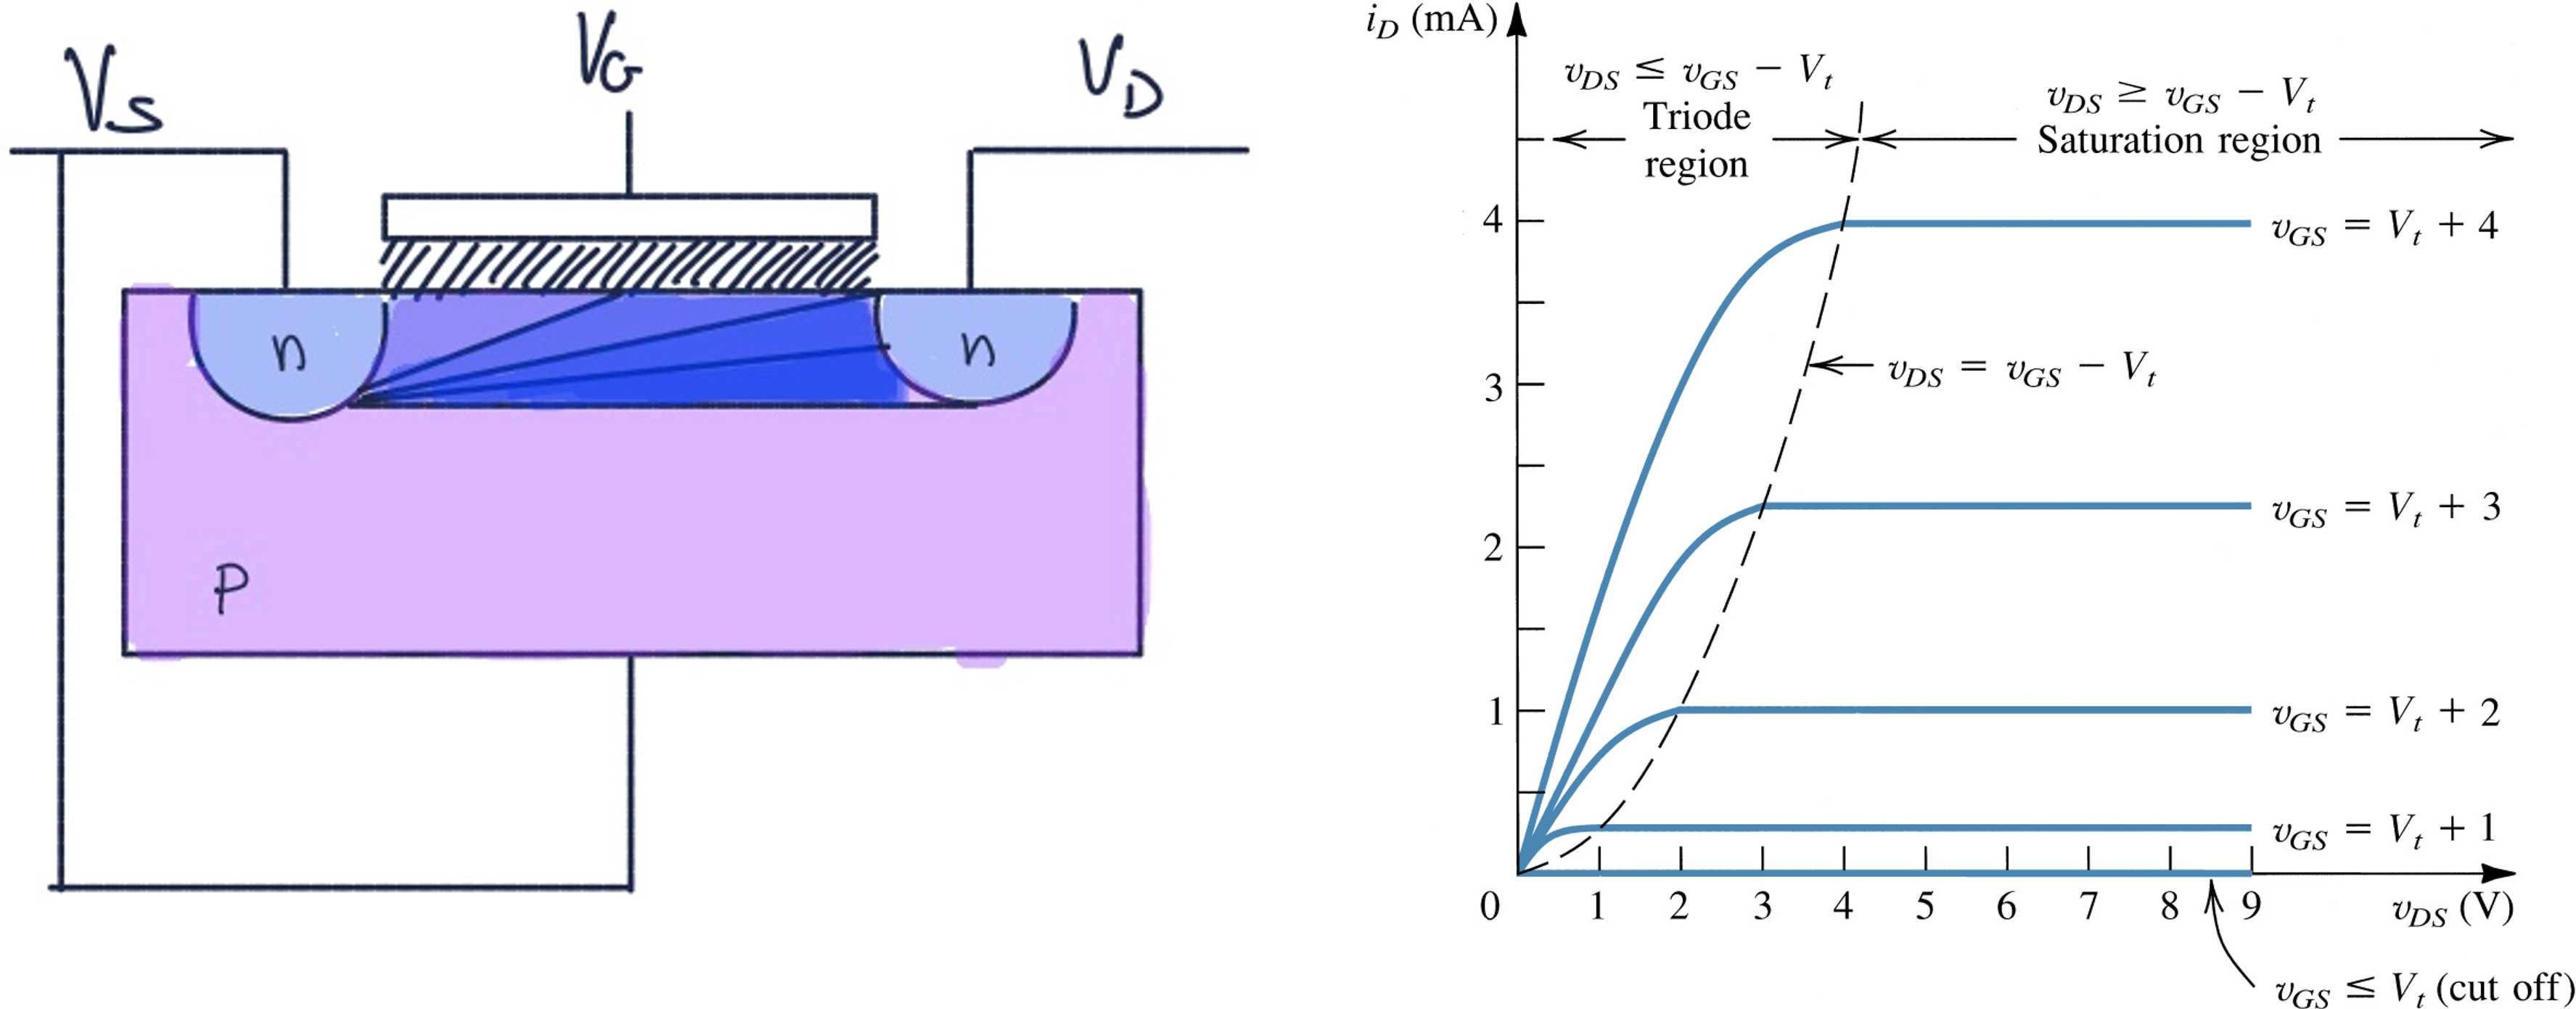
\includegraphics[width=0.6\paperwidth]{images/nmos idvds.png}
    \caption{A l'esquerra, els canals formats amb diferents regions en un transistor nMOS amb el Substrate connectat al Source, de menys a més fosc: sense canal, punt de contacte, regió triòdica i regió de saturació. A la dreta la gràfica $I_D(V_{DS})$ amb cada una de les regions.}
    \label{fig:nmos23}
\end{figure}

\begin{wrapfigure}{r}{0.25\paperwidth}
    \centering
    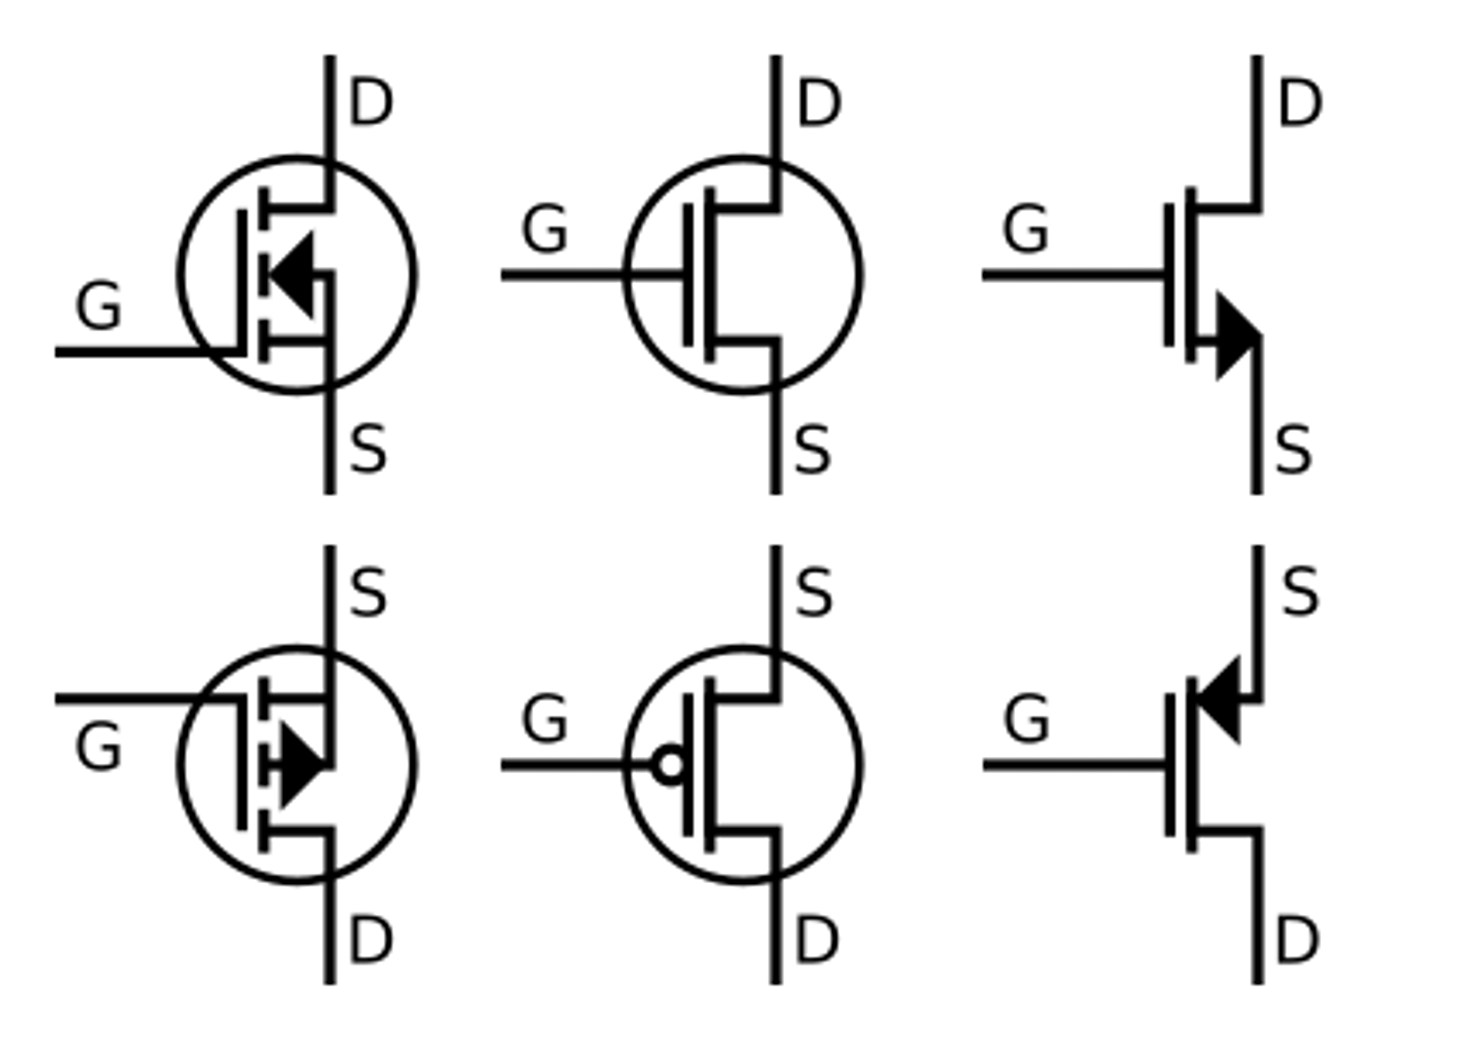
\includegraphics[width=\linewidth]{images/npmos symbols.png}
    \caption{Diferents símbols per representar nMOS (adalt) i pMOS (abaix)}
    \vspace{-2cm}
\end{wrapfigure}

\subsection{Estructura d'un CMOS, senyals 0 i 1, portes lògiques}

Sabent com funcionen els nMOS i pMOS podem utilitzar el seu funcionament per construir dispositius (portes) digitals.

Una porta constarà d'entrades i sortides. Realment, a part de les entrades i les sortides hi haurà una línea on tindrem sempre un voltatge alt (que serà el nostre \texttt{1}) i una línea amb voltatge baix (el \texttt{0}).

Els inputs d'entrada únicament determinarà l'activació de la porta, portant la creació o destrucció del canal.

Una porta lògica simple de modelar és la \texttt{NOT}, on presentarem la seva taula de la veritat i com es distribueix la corrent en cada mode de funcionament.

\begin{figure}[h]
    \centering
    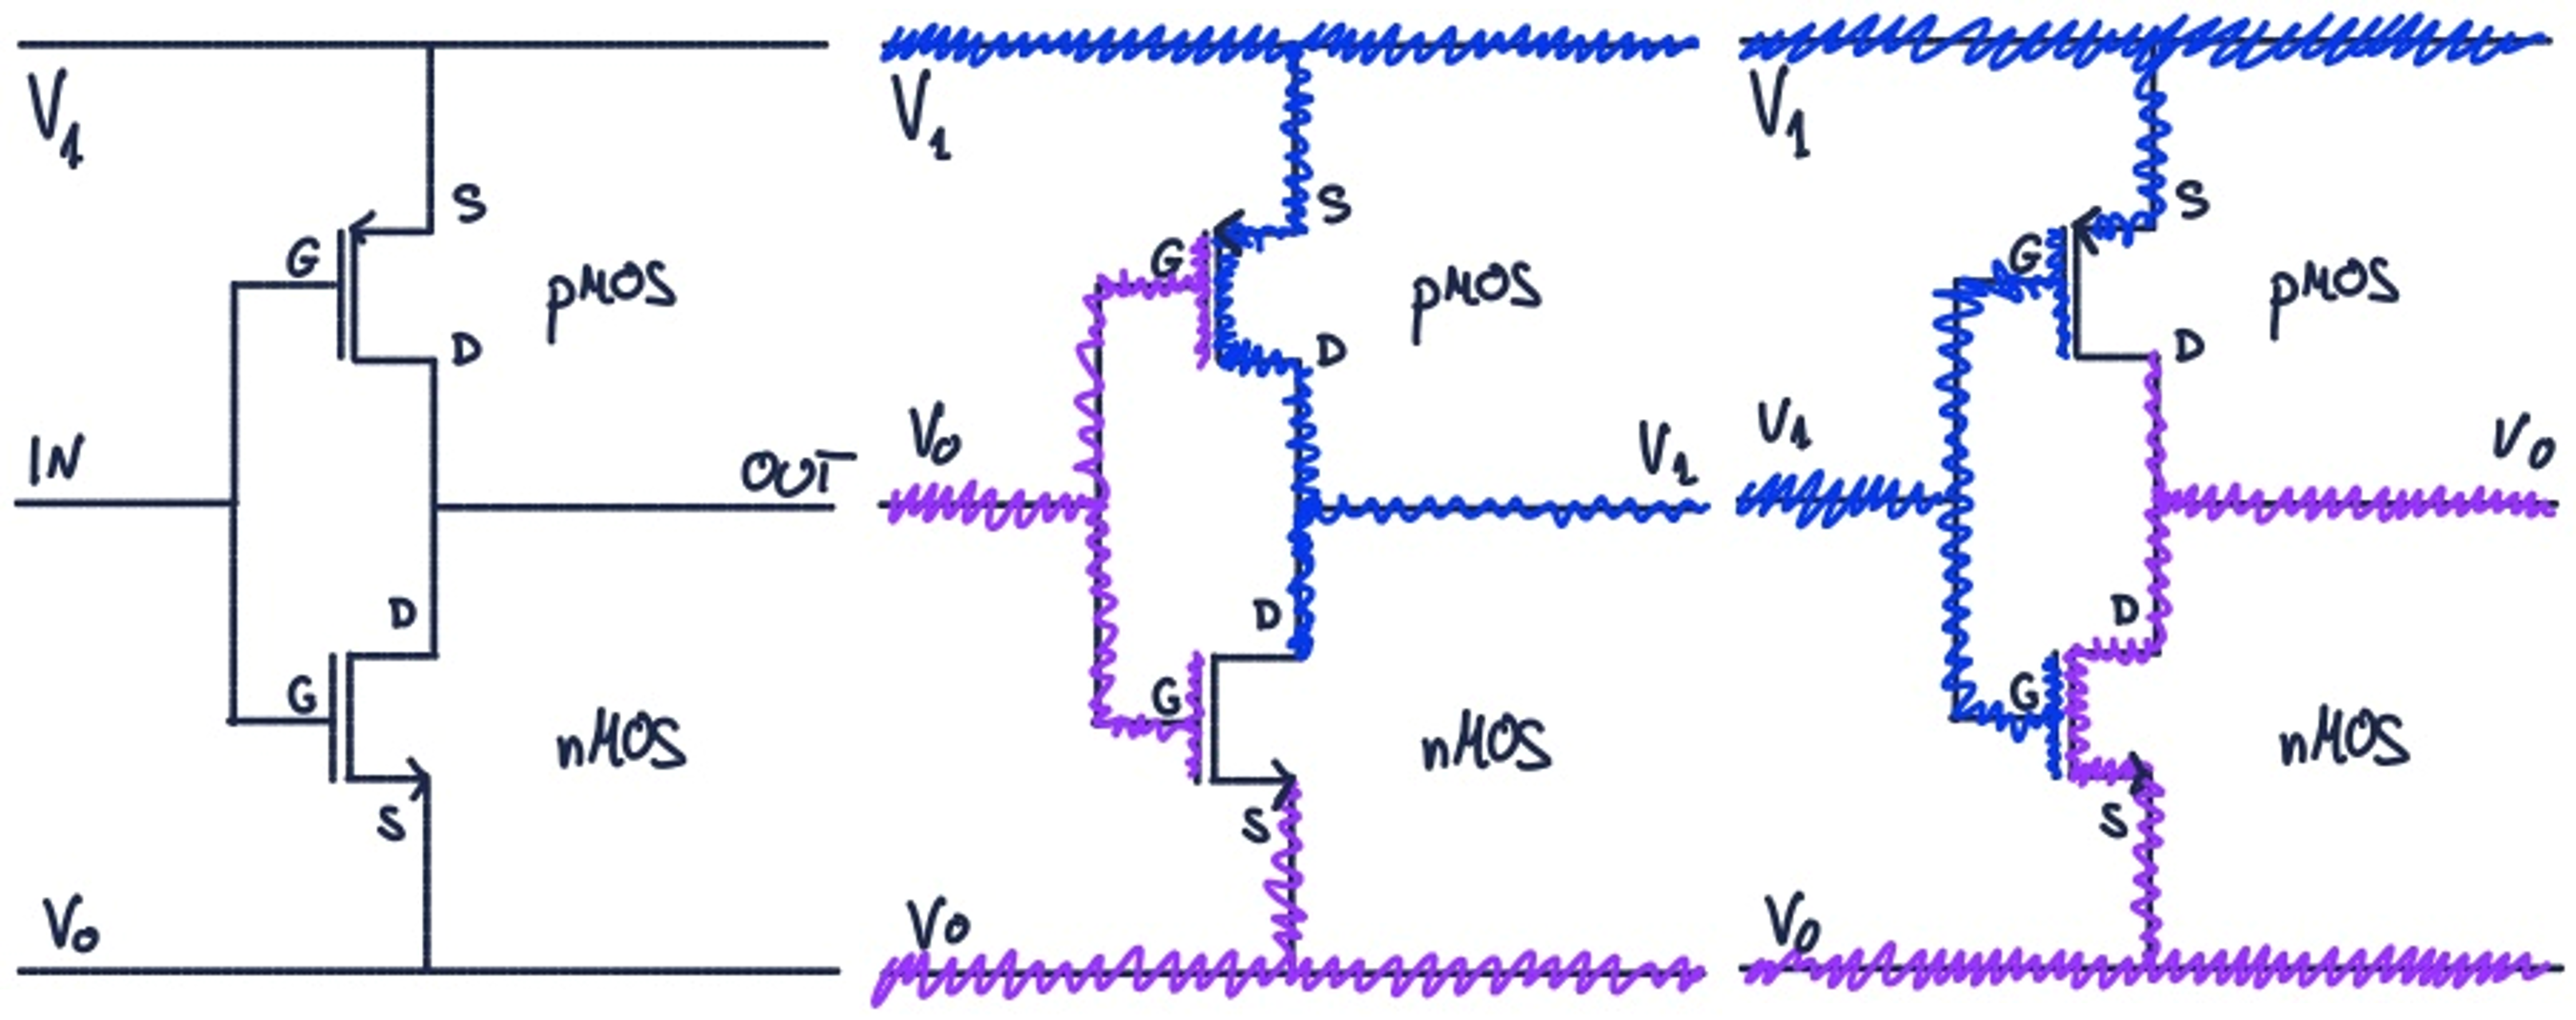
\includegraphics[width=0.7\textwidth]{images/notgate actions.png}
    \caption{Porta \texttt{NOT} amb les seves configuracions.}
    \label{fig:not-gate}
\end{figure}

Tenint present que els voltatges per definir 0 i 1 son tipicament $V_0 \approx \qty{0}{\volt}$ i $V_1 \approx \qty{5}{\volt}$ i que els voltatges d'umbral son aproximadament: $V_T^{nMOS} \approx \qty{1}{\volt} \quad V_T^{pMOS} \approx \qty{-1}{\volt}$.
\newpage
Les condicions per cada un dels dispositious son les vistes a la Taula \ref{tab:saturation-cond}. També existeixen les condicions de saturació i treball triòdic, que en aquest cas, com estem fent un estudi digital del dispositiu no entrarem en la resposta analògica d'aquest. 

\begin{table}[]
    \centering
    \begin{tabular}{c|c}
        \textbf{nMOS} & \textbf{pMOS} \\
        \hline
        $V_{GS} \ge V_{T}$ & $ \left|V_{GS}\right| \ge \left|V_{T}\right|$
    \end{tabular}
    \caption{Condicions de contacte pels pMOS i nMOS}
    \label{tab:saturation-cond}
\end{table}

Llavors, aplicant a cada cas.

\begin{table}[h]
    \centering
    \begin{tabular}{c|c|c}
        $V_{IN} = V_G$ & \textbf{nMOS} ($V_S = \qty{0}{\volt}$) & \textbf{pMOS} ($V_S = \qty{5}{\volt}$) \\
        \hline
        $V_0 = 0V$ & $V_{GS} = 0 \rightarrow \text{NO CONTACTE} $ & $V_{GS} = -5 \rightarrow \text{CONTACTE}$\\
        $V_1 = 5V$ & $V_{GS} = 5 \rightarrow \text{CONTACTE} $ & $V_{GS} = 0 \rightarrow \text{NO CONTACTE}$
    \end{tabular}
    \label{<label>}
\end{table}

On podem veure les connexions que es fan a la Figura \ref{fig:not-gate}. A partir d'ara, pensant només en l'electrònica digital, podem veure els pMOS com interruptors que amb senyal 0 estaràn tancats i amb senyal 1 estaràn oberts, i els nMOS al contrari, si te senyal 0 estaràn oberts, i si te senyal 1 estaràn tancats.

\subsection{Construcció de la porta universal \texttt{NAND}, taula de la veritat i altres portes a partir de \texttt{NAND} }

A continuació presentarem la porta \texttt{NAND}. Aquest aporta té un caràcter universal ja que es poden construir tot tipus de circuits només utilitzant aquesta. També hi ha la porta \texttt{NOR} que també te la mateixa característica universal.

\begin{figure}[h!]
    \centering
    \begin{minipage}[t]{0.7\textwidth}
        \centering
        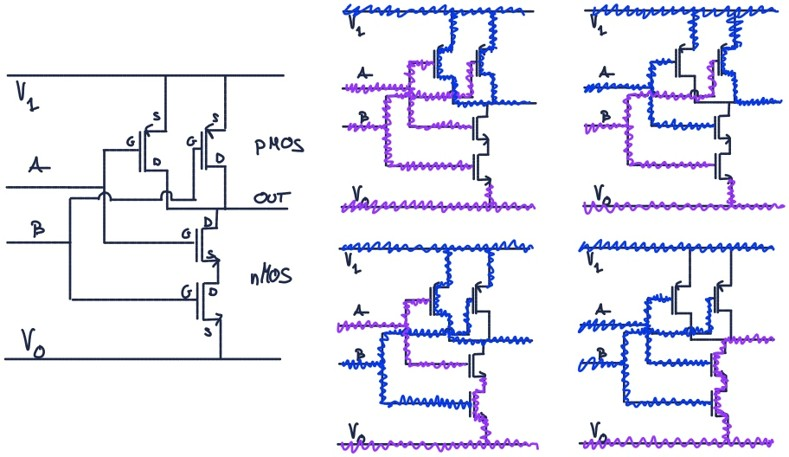
\includegraphics[width=\linewidth]{images/nand.jpg}
        \label{fig:nand}
    \end{minipage}
    \hfill
    \begin{minipage}[t]{0.25\textwidth}
    \centering
    \vspace{-4.7cm}
    \begin{tabular}{cc|c}
      \textbf{A} & \textbf{B} & \textbf{OUT} \\
      \hline
      0 & 0 & 1 \\
      0 & 1 & 1 \\
      1 & 0 & 1 \\
      1 & 1 & 0 \\
    \end{tabular}
    \label{tab:nand}
  \end{minipage}
    \caption{Porta \texttt{NAND} a l'esquerra amb tecnologia CMOS, casos d'us al mig, taula de la veritat a la dreta.}
  
\end{figure}

Finalment introduirem les tres portes lògiques bàsiques: \texttt{AND}, \texttt{OR} i \texttt{NOT} construides a partir de la lògica \texttt{NAND} a la Figura \ref{fig:portes}.

\begin{figure}[H]
  \centering
    \begin{minipage}{0.7\textwidth}
    \centering
  \begin{subfigure}[t]{0.3\textwidth}
    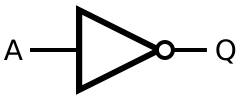
\includegraphics[width=\linewidth]{images/NOT_ANSI_Labelled.svg.png}
  \end{subfigure}
  \hfill
  \begin{subfigure}[t]{0.3\textwidth}
    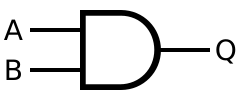
\includegraphics[width=\linewidth]{images/AND_ANSI_Labelled.svg.png}
  \end{subfigure}
  \hfill
  \begin{subfigure}[t]{0.3\textwidth}
    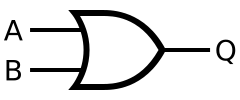
\includegraphics[width=\linewidth]{images/OR_ANSI_Labelled.svg.png}
  \end{subfigure}
  

  \vspace{1em}

  
  \begin{subfigure}[t]{0.3\textwidth}
    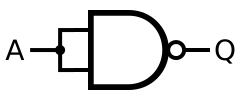
\includegraphics[width=\linewidth]{images/NOT_from_NAND.svg.png}
    \caption{Porta \texttt{NOT}}
  \end{subfigure}
  \hfill
  \begin{subfigure}[t]{0.3\textwidth}
    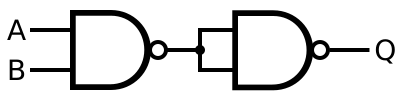
\includegraphics[width=\linewidth]{images/AND_from_NAND.svg.png}
    \caption{Porta \texttt{AND}}
  \end{subfigure}
  \hfill
  \begin{subfigure}[t]{0.3\textwidth}
    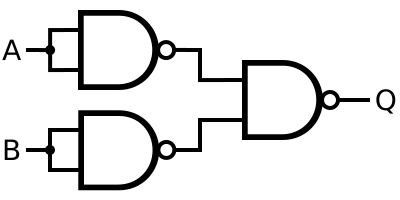
\includegraphics[width=\linewidth]{images/OR_from_NAND.svg.png}
    \caption{Porta \texttt{OR}}
  \end{subfigure}
\end{minipage}
  

  \caption{Portes digitals. Adalt símbol ANSI, abaix representació en la lógica \texttt{NAND}.}
  \label{fig:portes}
\end{figure}


\section{Aplicacions}

Deixant de banda les aplicacions més obvies que poden tenir els CMOS, com poden ser la creació de microprocessadors amb la vinguda de tota l'era digital, presentarem una serie d'aplicacions més indirectes, tot i formar part molt 

\subsection{Astronomia}
\subsection{Medicina}

% \subsection{Portes lògiques}

% \subsection{Sensors i cameres digitals}
% % Cámaras digitales, sensores industriales, robótica.

\printbibliography

\end{document}
